\documentclass[notes=show,handout]{beamer}
\usepackage{amsmath}
\usepackage{graphicx}
\usepackage{mathpazo}
\usepackage{hyperref}
\usepackage{multimedia}
\usepackage{epstopdf}
\usepackage{tikz}
\usetikzlibrary{shapes,backgrounds}
\usepackage{multicol}

\setcounter{MaxMatrixCols}{10}
\usetheme{Madrid}


\newtheorem{conj}{Conjecture}[section]
\newtheorem{aim}{Aim}[section]
\newtheorem{remark}{Remark}[section]
\newtheorem{proposition}{Proposition}[section]
\newtheorem{interpretation}{Interpretation}[section]
\newtheorem{goal}{Goal}[section]
\newtheorem{exercise}{Exercise}[section]



\newcommand{\mbf}[1]{\mathbf{#1}}
\newcommand{\beq}{\begin{equation}}
\newcommand{\eeq}{\end{equation}}
\newcommand{\bea}{\begin{eqnarray}}
\newcommand{\eea}{\end{eqnarray}}
\newcommand{\ba}{\begin{array}}
\newcommand{\ea}{\end{array}}
\newcommand{\bi}{\begin{itemize}}
\newcommand{\ei}{\end{itemize}}
\newcommand{\ben}{\begin{enumerate}}
\newcommand{\een}{\end{enumerate}}
\newcommand{\nn}{\nonumber}
\newcommand{\fn}[1]{\footnote{#1}}
\renewcommand{\r}{\right}
\renewcommand{\l}{\left}
\long\def\symbolfootnote[#1]#2{\begingroup\def\thefootnote{\fnsymbol{footnote}}\footnote[#1]{#2}\endgroup}


\definecolor{darkGSEM}{RGB}{70,95,127}
\definecolor{darkGSEM2}{RGB}{40,80,150}
\definecolor{GSEM}{RGB}{96,121,153} % GSEM 10% lighter

%%% Global colors
\setbeamercolor*{palette primary}{use=structure,fg=white,bg=darkGSEM}
\setbeamercolor*{palette quaternary}{use=structure,fg=white,bg=darkGSEM!90}
\setbeamercolor{frametitle}{fg=white,bg=GSEM!80}

%%% TOC colors
\setbeamercolor{section in toc}{fg=darkGSEM}

%%% itemize colors
\setbeamertemplate{itemize items}[circle]
\setbeamercolor{itemize item}{fg=darkGSEM2}
\setbeamercolor{itemize subitem}{fg=darkGSEM2}
\setbeamercolor{itemize subsubitem}{fg=darkGSEM2}


%%% enumerate colors
\setbeamercolor{item projected}{fg=white,bg=GSEM}
\setbeamertemplate{enumerate item}{\insertenumlabel.}
\setbeamercolor{enumerate item}{fg=darkGSEM2}
\setbeamercolor{enumerate subitem}{fg=darkGSEM2}
\setbeamercolor{enumerate subsubitem}{fg=darkGSEM2}


\AtBeginSection[]
{
  \begin{frame}
    \frametitle{Outline}
    \tableofcontents[currentsection]
  \end{frame}
}





\begin{document}

\title[S110015]{Probability I}
\subtitle{Lecture 1}
\author[La Vecchia]{Davide La Vecchia}
\date{Spring Semester 2020}
\maketitle



\begin{frame}
\frametitle{Definitions}

In this course we are going to need also some elements of \color{blue} set theory.\color{black}\\

To start our journey, let us introduce some definitions.

\begin{definition}
A random experiment  is a process that can result in two or more different outcomes with uncertainty as to which will be observed.
\end{definition}

\begin{definition}
An event is an uncertain outcome of a random experiment. An event can be
\begin{itemize}
\item Elementary: it includes only one particular outcome of the experiment
\item Composite: it includes more than one elementary outcome in the possible sets of outcomes.
\end{itemize}
\end{definition}

\end{frame}



\begin{frame}
\frametitle{Definitions}


\begin{definition}
The sample space is the complete listing of the elementary events that can occur in a random experiment. We will denote
the sample space by $S$.
\end{definition}

%\end{frame}


%\begin{frame}
%\frametitle{Random experiments (cont'd)}

\begin{example}

\begin{figure}[h!]
\centering
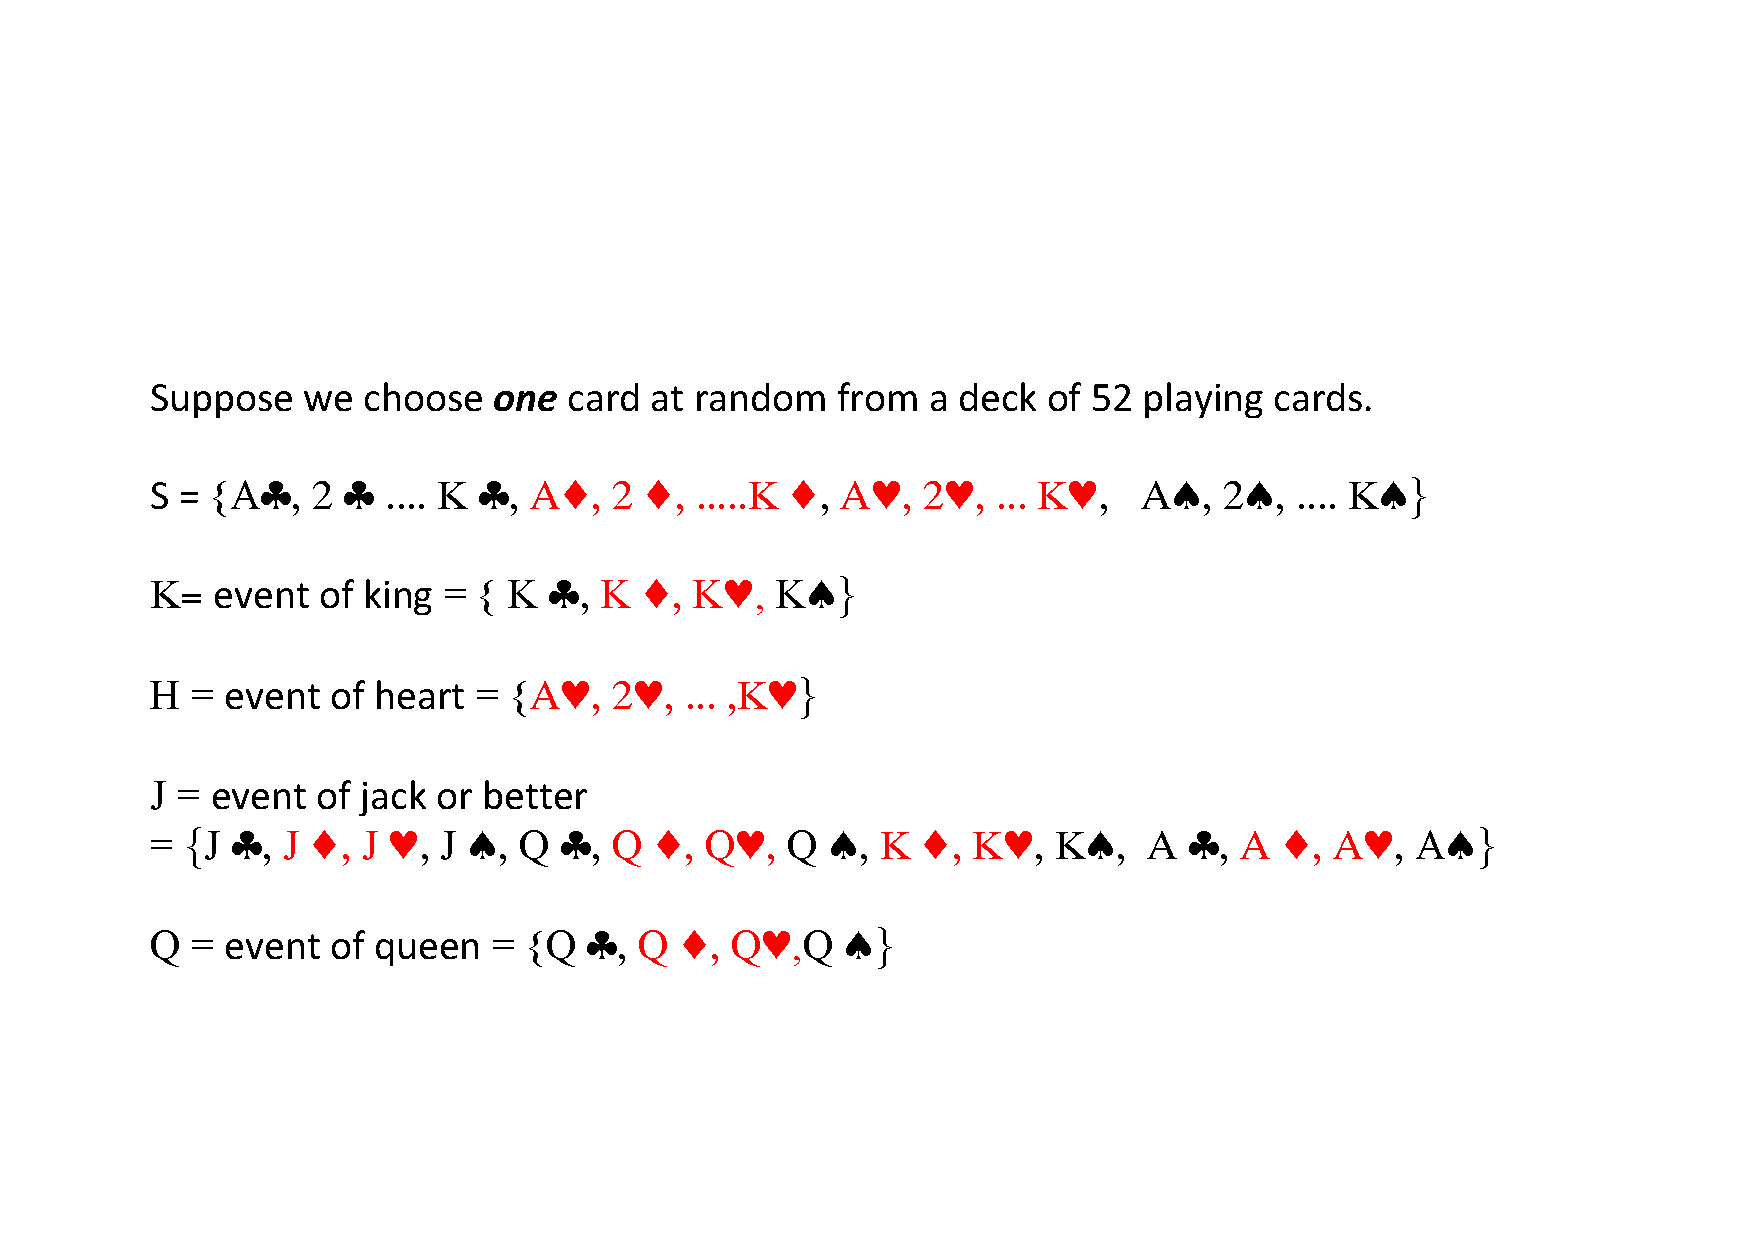
\includegraphics[width=0.9\textwidth,height=0.55\textheight]{Example1_GE.pdf}
\end{figure}
\end{example}
\end{frame}

\begin{frame}
\frametitle{Definitions}
\begin{example}
\begin{itemize}
\item If we flip two coins (experiment) we have, for each coin,
\begin{itemize}
\item $H$ for Head
\item $T$ for Tail
\end{itemize}
so the sample space contains the following four points

$$
S = \{ (HH),(HT),(TH),(TT)  \}.
$$

\item If the experiment consists in measuring (in hours) the life time of a your iPhone, the sample space consists of all nonnegative real
numbers:
$$
S = \{x: 0 \leq x < \infty \}
$$

or, equivalently, $S\equiv \mathbb{R}^+$.
\end{itemize}



\end{example}
\end{frame}


\begin{frame}
\frametitle{Some definitions from set theory}
To deal with events, we rely on the set theory. Some definitions:
\begin{definition}
\begin{itemize}
\item If every element of a set $A$ is also an element of a set $B$, then $A$ is defined to be a \textit{subset} of $B$, and we will write
$$ A \subset B$$
and we read it as ``$A$ is contained in $B$''
\item Two sets $A$ and $B$ are defined to be equal if
$$A \subset B \text{ \ and \ } B \subset A;$$
\item If a set $A$ contains no points, it will be called the \textit{null set, or empty set}, and it is typically denoted by $\varnothing$.
\end{itemize}


\end{definition}


\end{frame}


%\begin{frame}
%\frametitle{Some definitions from set theory}
%
%
%\end{frame}

\begin{frame}
\frametitle{Elements of set theory (Venn diagram)}

A Venn diagram is an enclosed figure representing the sample space with one or more events defined.

\begin{figure}[h!]
\centering
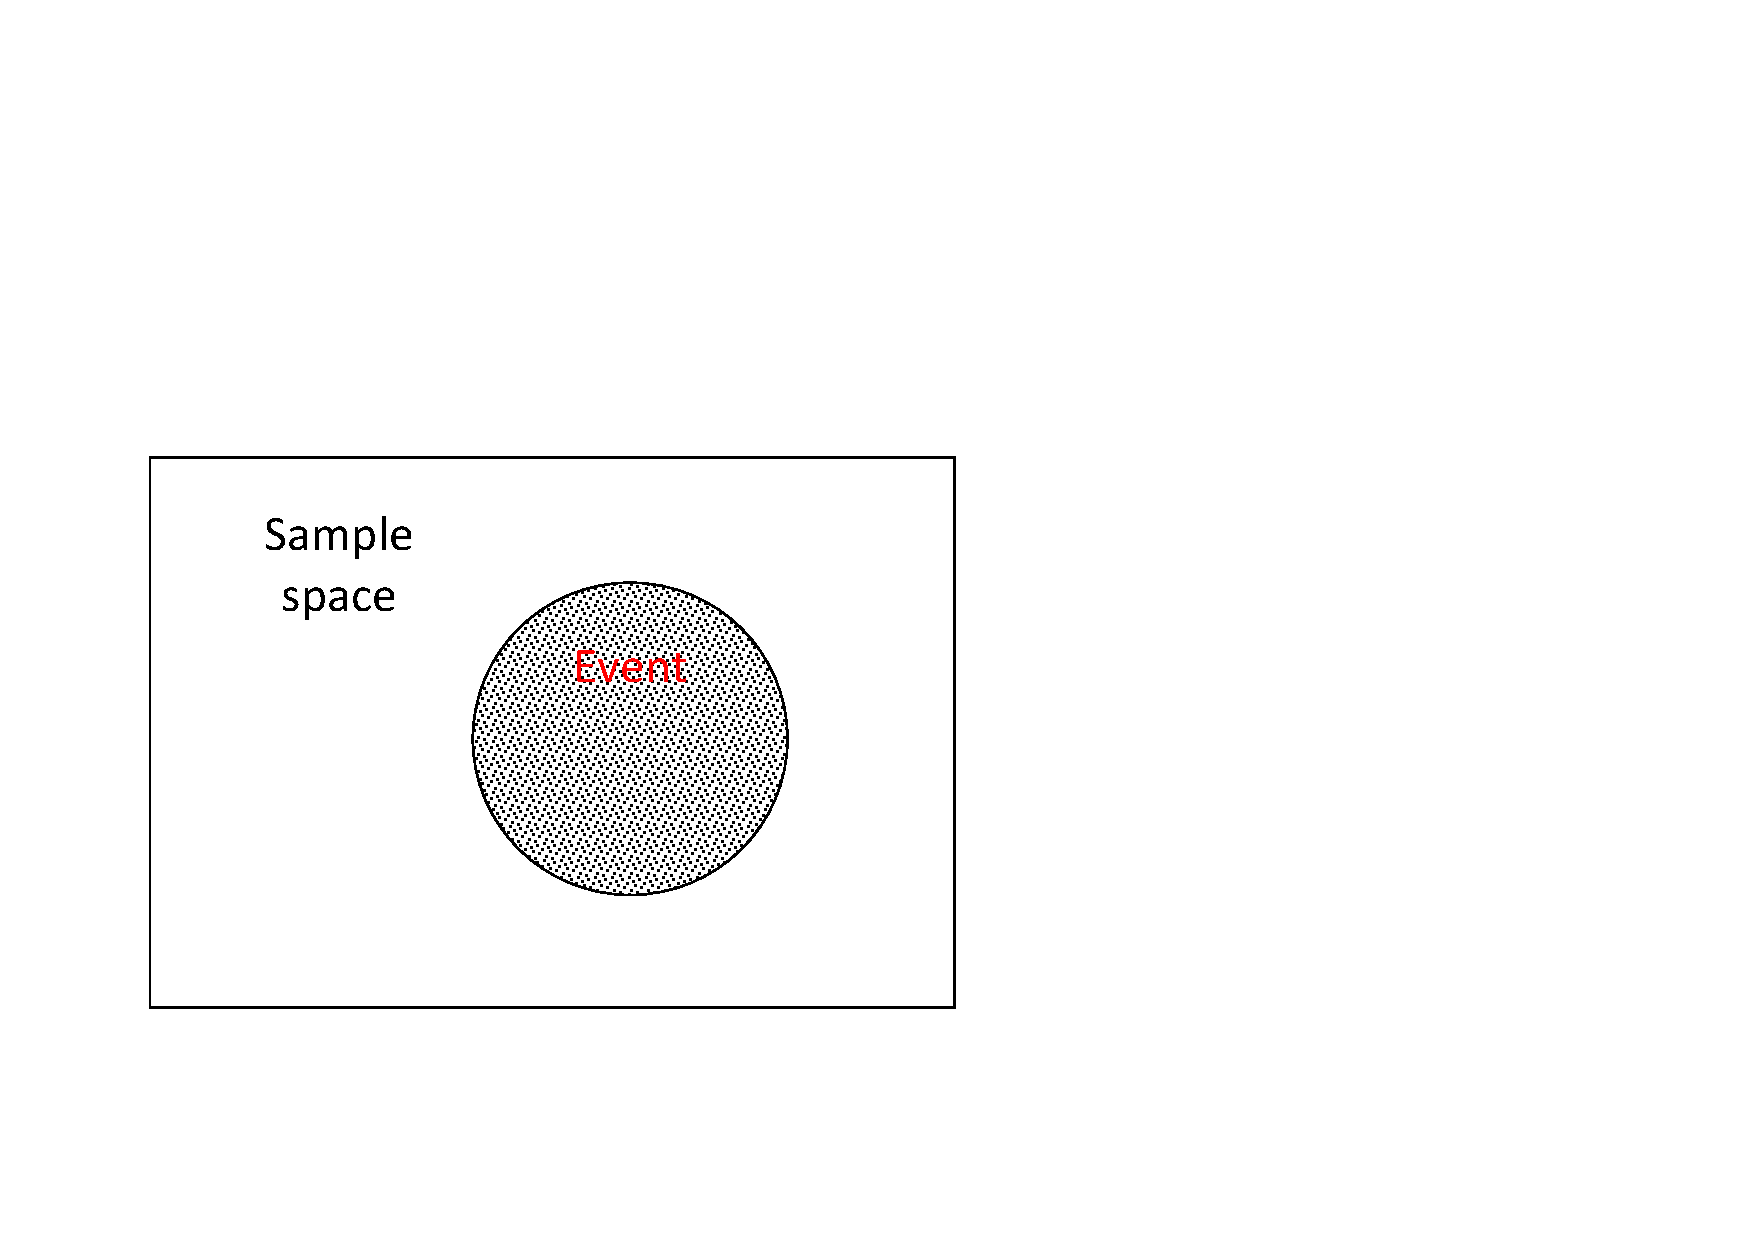
\includegraphics[width=0.8\textwidth,height=0.6\textheight]{Venn1.pdf}
\end{figure}
\end{frame}


\begin{frame}
\frametitle{Elements of set theory (Venn diagram)}


Two events are mutually exclusive is they cannot occur jointly...


\begin{figure}[h!]
\centering
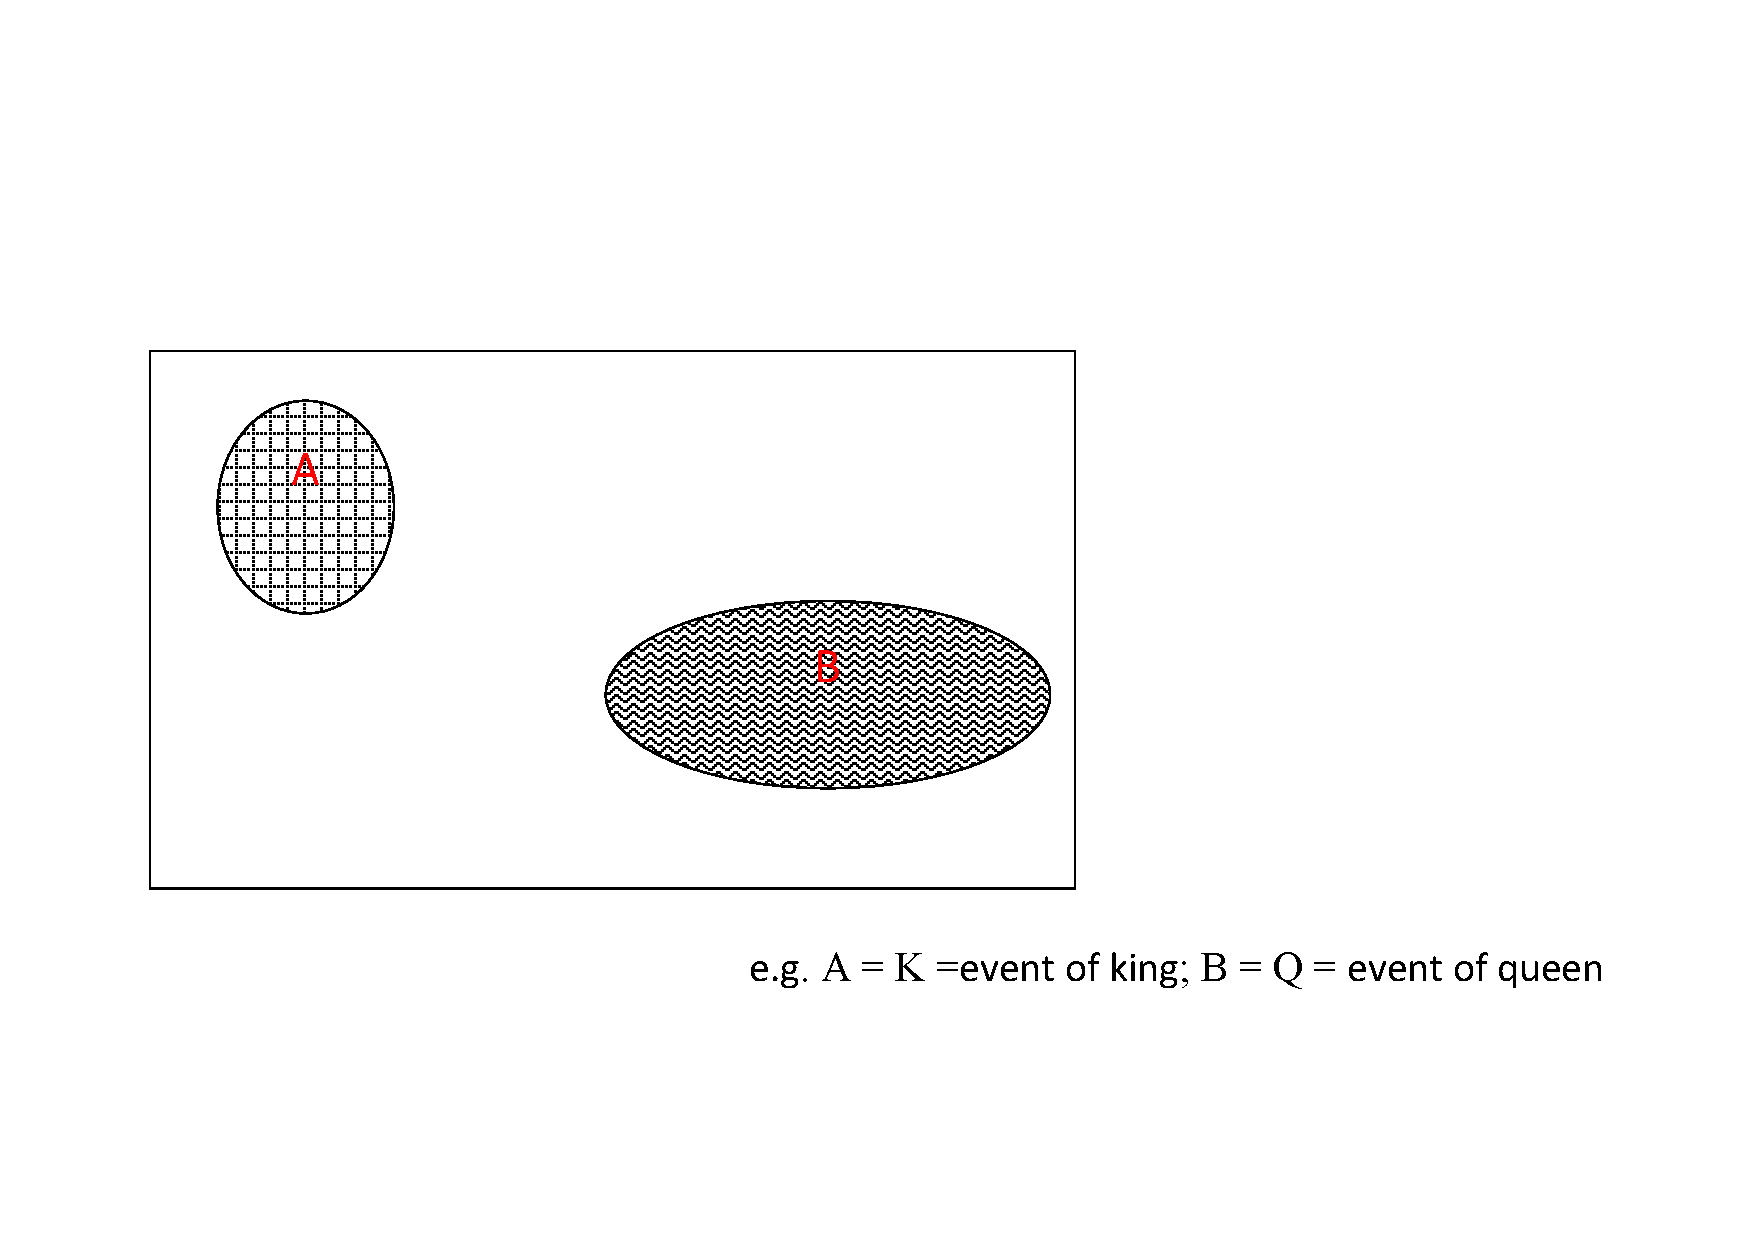
\includegraphics[width=1\textwidth,height=0.7\textheight]{Venn2.pdf}
\end{figure}
\end{frame}

\begin{frame}
\frametitle{Elements of set theory (Venn diagram)}

... and not mutually exclusive ...


\begin{figure}[h!]
\centering
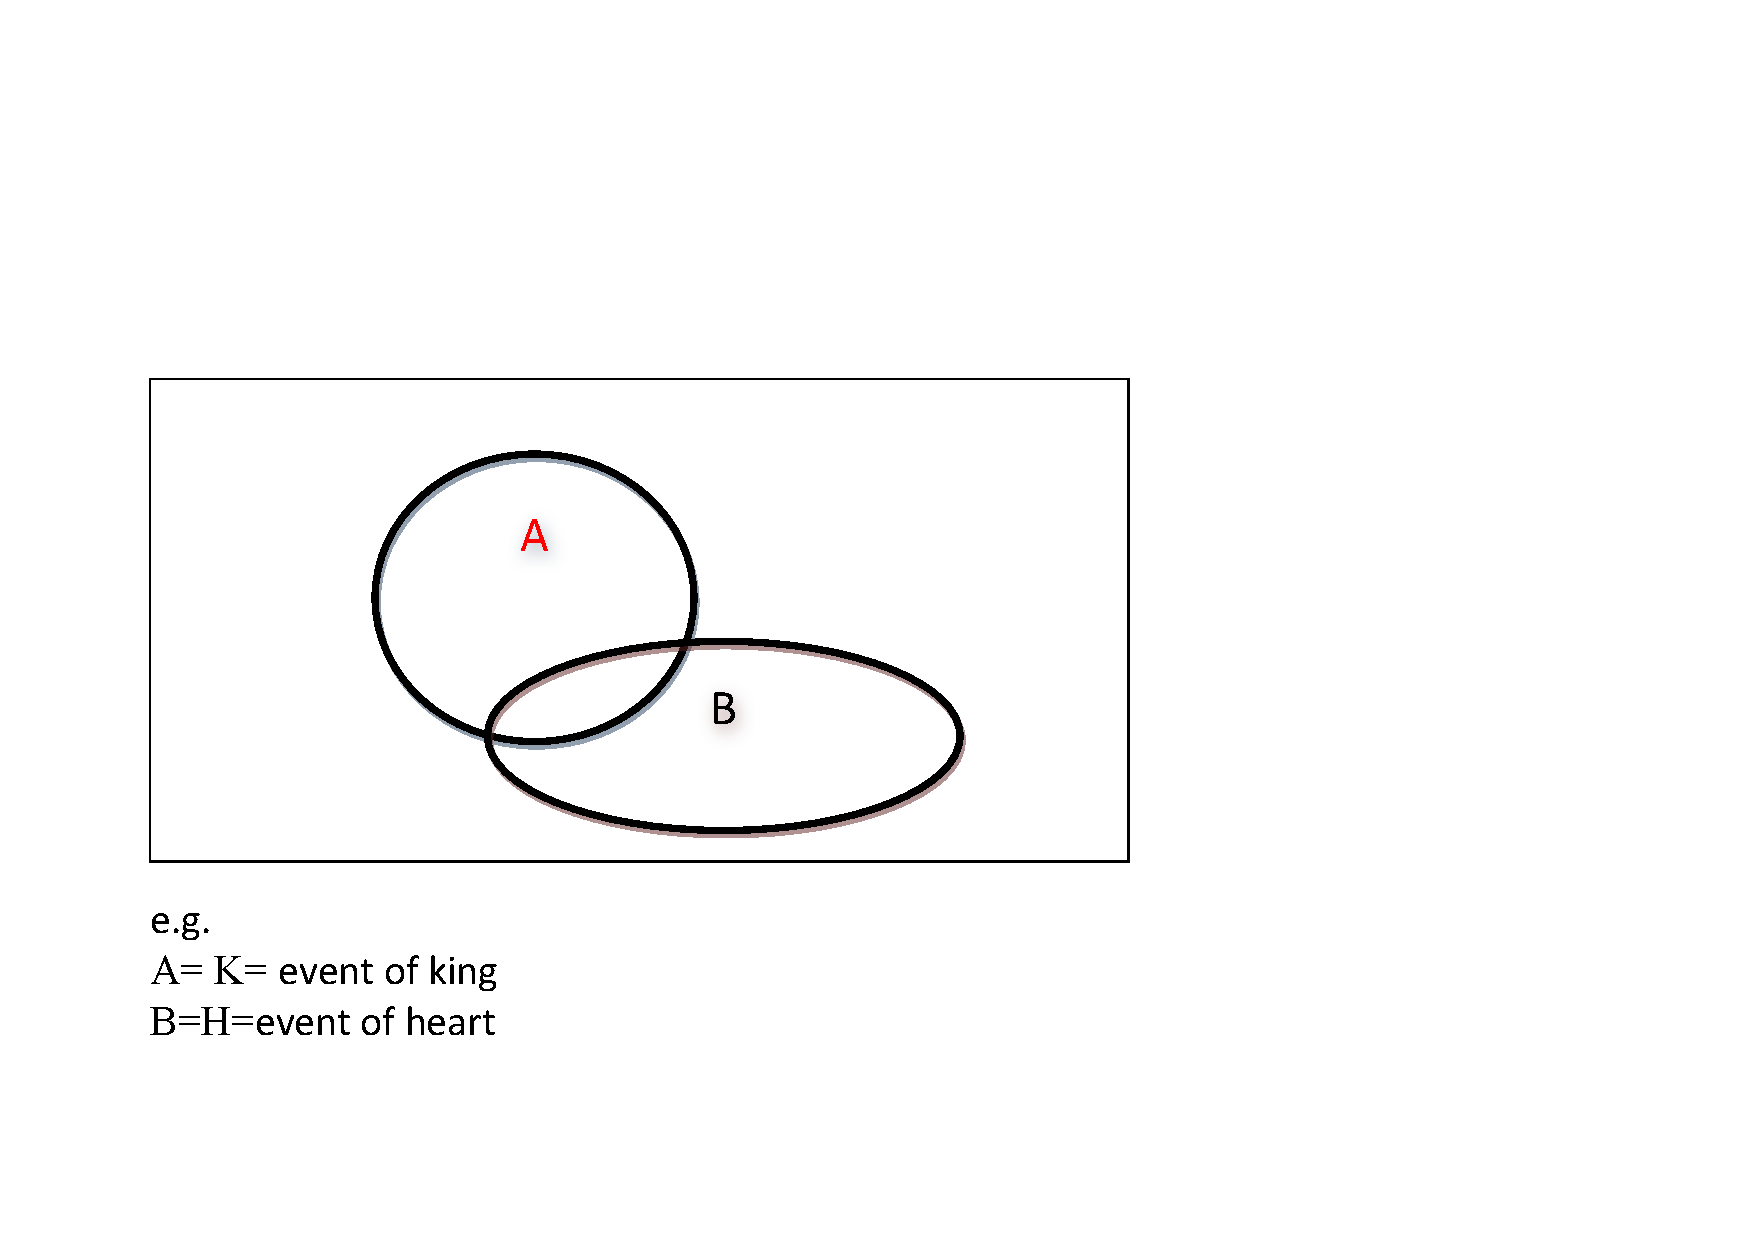
\includegraphics[width=1\textwidth,height=0.7\textheight]{Venn3.pdf}
\end{figure}
\end{frame}


\begin{frame}
\frametitle{Elements of set theory (Venn diagram)}

The union of the events $A$ and $B$ is the event which occurs when either $A$ or $B$ occurs: $A \cup B$ \\
%\begin{figure}[h!]
%\centering
%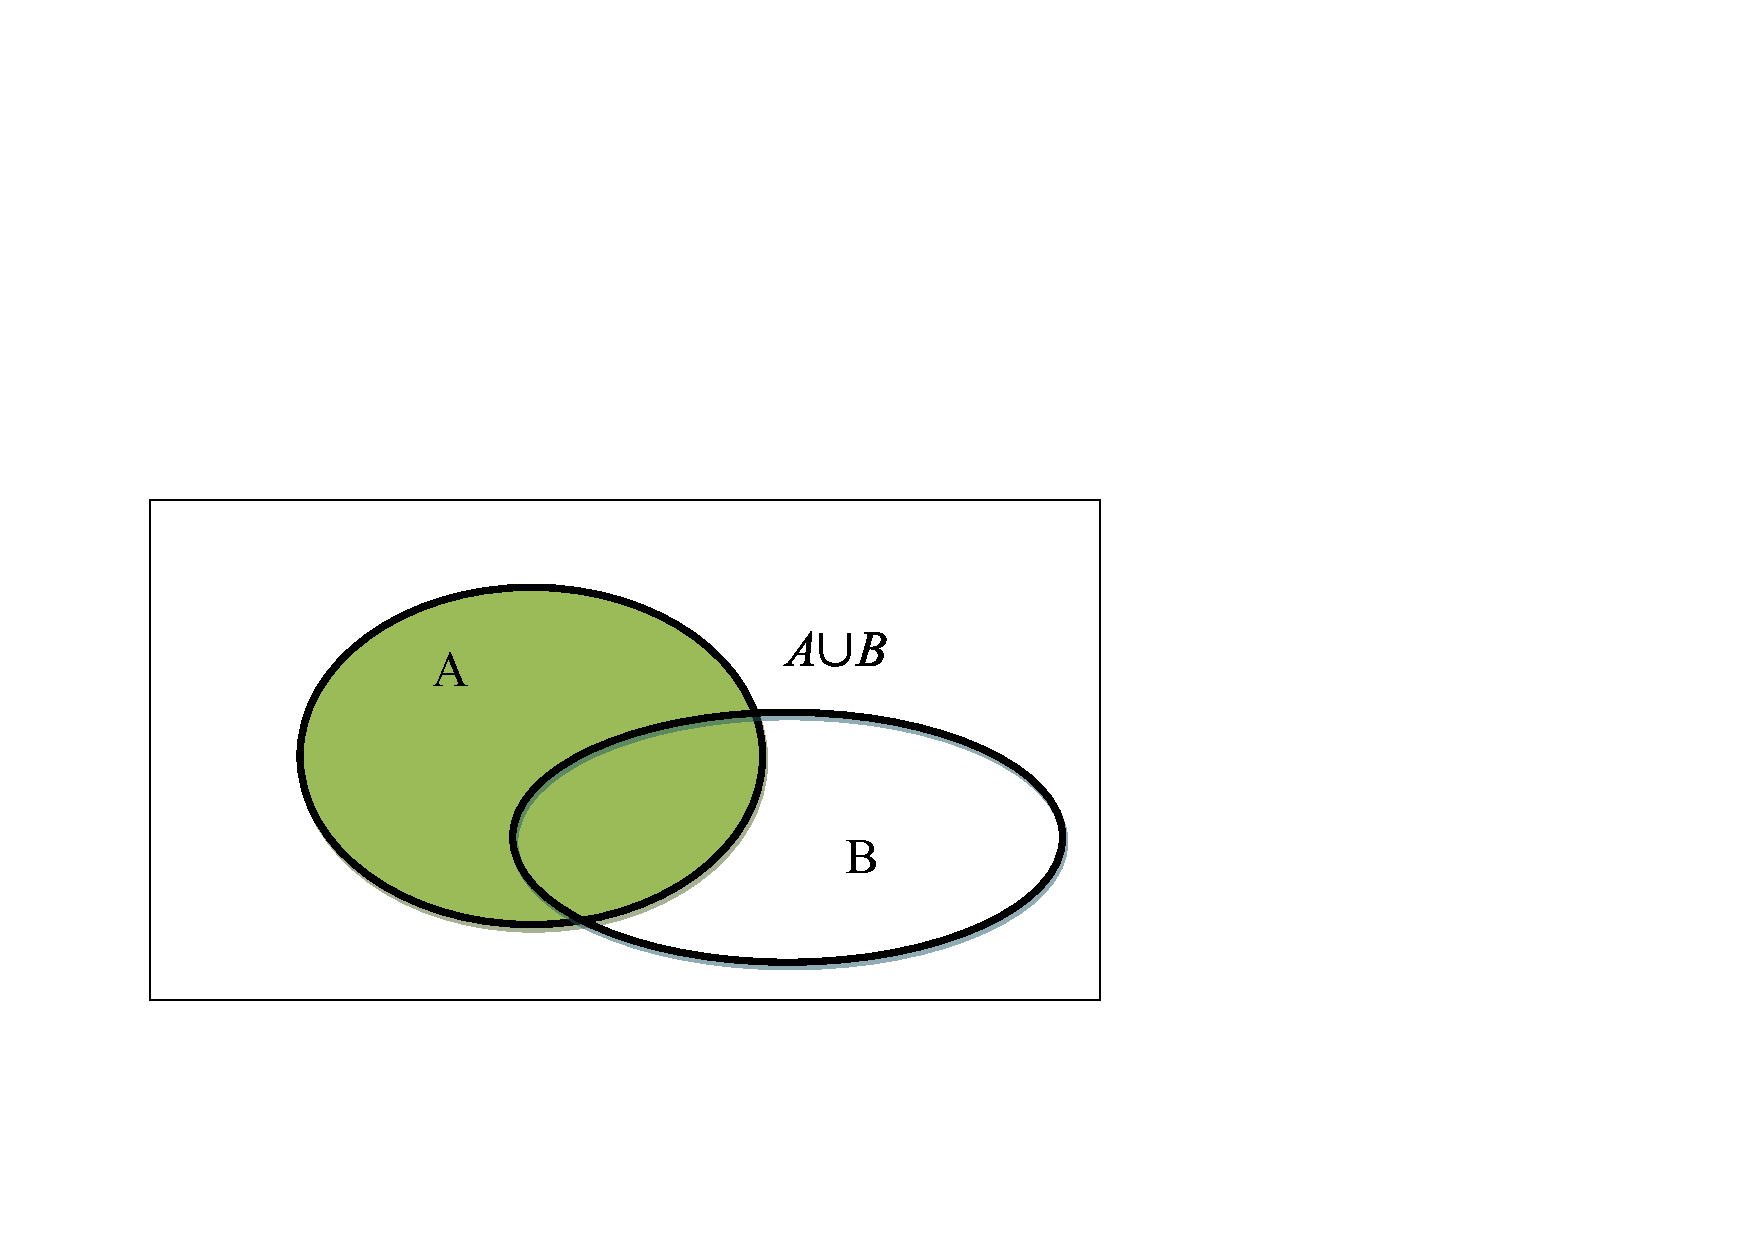
\includegraphics[width=1\textwidth,height=0.7\textheight]{Venn4.pdf}
%\end{figure}
\vspace{1cm}
\hspace{2cm}
\def\firstcircle{(0,0) circle (1.5cm)}
\def\secondcircle{(45:2cm) circle (1.5cm)}
\begin{tikzpicture}
    \begin{scope}[shift={(6cm,5cm)}, fill opacity=0.65]
        \fill[blue!20] \firstcircle;
        \fill[blue!20] \secondcircle;
        \draw \firstcircle node[below] {$A$};
        \draw \secondcircle node [above] {$B$};
%        \draw node [above] {$A \cup B$}
    \end{scope}
\end{tikzpicture}

\end{frame}


\begin{frame}
\frametitle{Elements of set theory (Venn diagram)}

The intersection of the events $A$ and $B$ is the event which occurs when both $A$ and $B$ occur: $A \cap B$\\
\vspace{1cm}
\hspace{2cm}
\def\firstcircle{(0,0) circle (1.5cm)}
\def\secondcircle{(45:2cm) circle (1.5cm)}
\begin{tikzpicture}
    \begin{scope}[shift={(6cm,5cm)}, fill opacity=0.65]
    \draw \firstcircle node[below] {$A$};
    \draw \secondcircle node [above] {$B$};

      \clip \firstcircle;
      \fill[blue!20] \secondcircle;
    \end{scope}
\end{tikzpicture}

\end{frame}


%\begin{frame}
%\frametitle{Elements of set theory (Venn diagram)}
%
%The intersection of the events $A$ and $B$ is the event which occurs when both $A$ and $B$ occur: $A \cap B$
%
%\begin{figure}[h!]
%\centering
%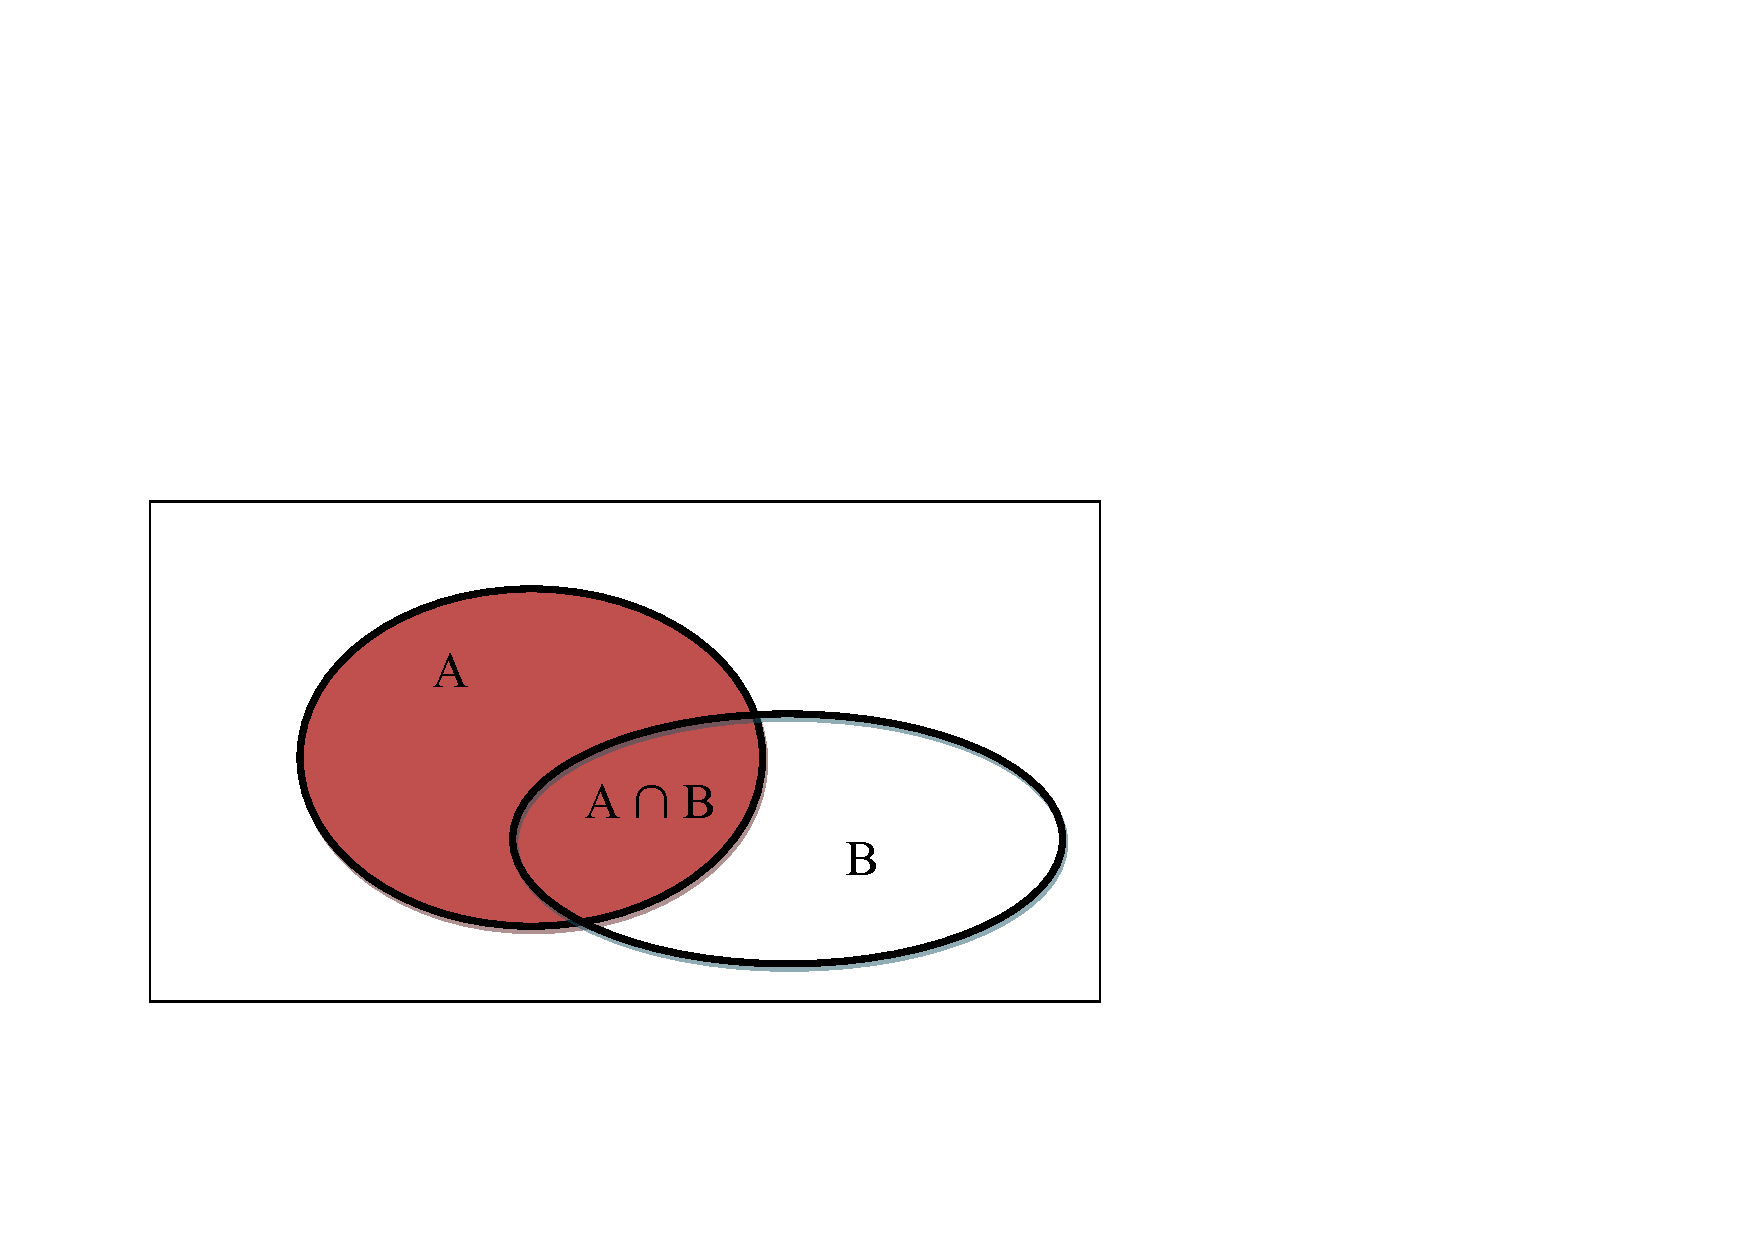
\includegraphics[width=1\textwidth,height=0.7\textheight]{Venn5.pdf}
%\end{figure}
%\end{frame}


\begin{frame}
\frametitle{Elements of set theory (Venn diagram)}

The complement of an event $A$ is the event which occurs when $A$ does not occur: $A^{c}$ (or $\overline{A}$)
\begin{figure}[h!]
\centering
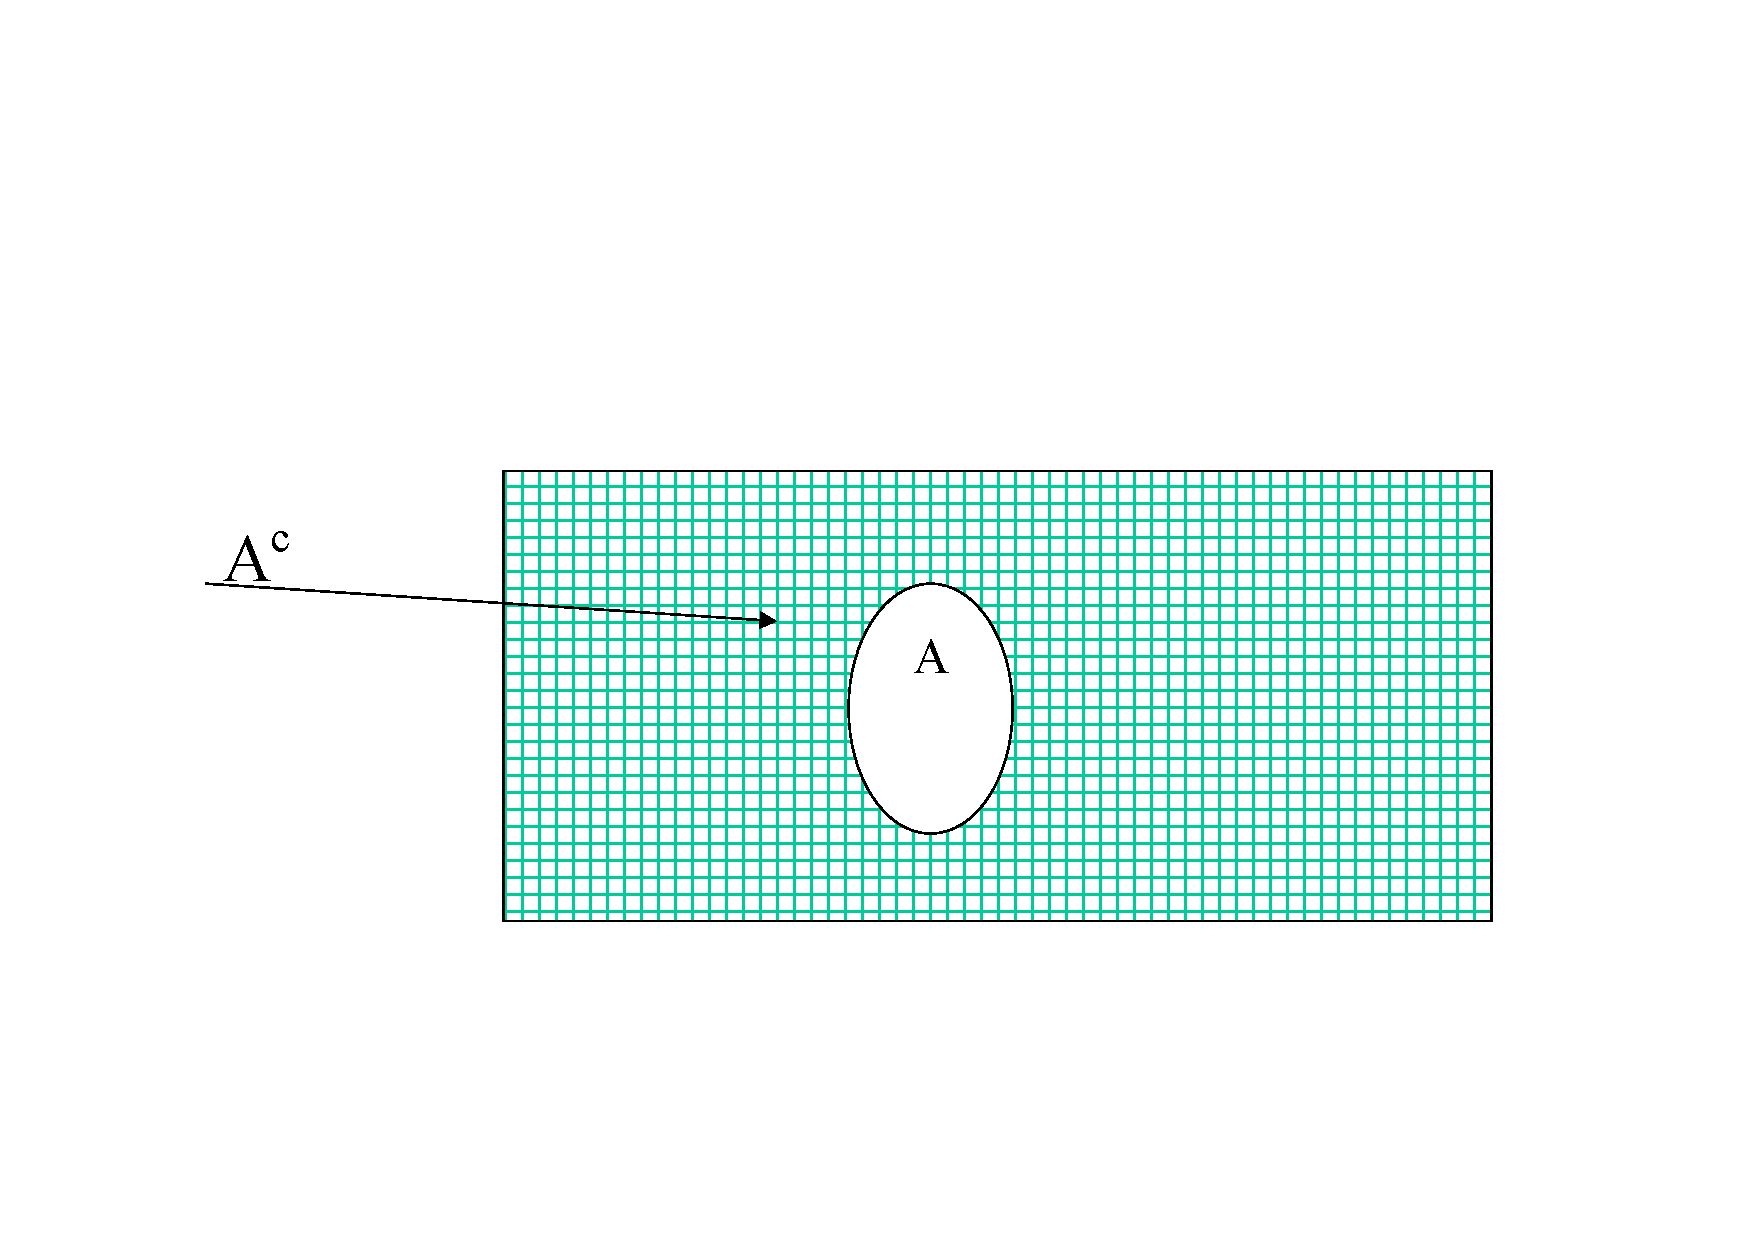
\includegraphics[width=0.8\textwidth,height=0.5\textheight]{Venn6.pdf}
\end{figure}
Let $S$ be the complete set of all possible events. Then, $A^c$ is such that $A \cup A^c = S$, or equivalently $A^c = S \setminus A = S-A$.
\end{frame}


\begin{frame}

\frametitle{Elements of set theory (Venn diagram)}

Let $A$, $B$, and $D$ be sets. The following laws hold:

\vspace{0.5cm}

\begin{itemize}

\item \textbf{Commutative laws}:
\begin{eqnarray*}
A \cup B = B \cup A \\
A \cap B = B \cap A
\end{eqnarray*}

\item \textbf{Associative laws}:
\begin{eqnarray*}
A \cup (B \cup D) = (A \cup B) \cup D \\
A \cap (B \cap D) = (A \cap B) \cap D
\end{eqnarray*}


\item \textbf{Distributive laws}:
\begin{eqnarray*}
A \cap (B \cup D) = (A \cap B) \cup (A\cap D)\\
A \cup (B \cap D) = (A\cup B) \cap (A \cup D)
\end{eqnarray*}

\end{itemize}

... verify them using Venn diagrams ...

\end{frame}

\begin{frame}
\frametitle{Elements of set theory (Venn diagram)}
... for instance, let $A_1, A_2, A_3$ be in $S$ and let us introduce the shorthand notation:
$$A_1 A_2 = A_1 \cap A_2  \quad \text{and} \quad A_1 A_3 = A_1 \cap A_3$$
Then, we have:
\begin{figure}[h!]
\centering
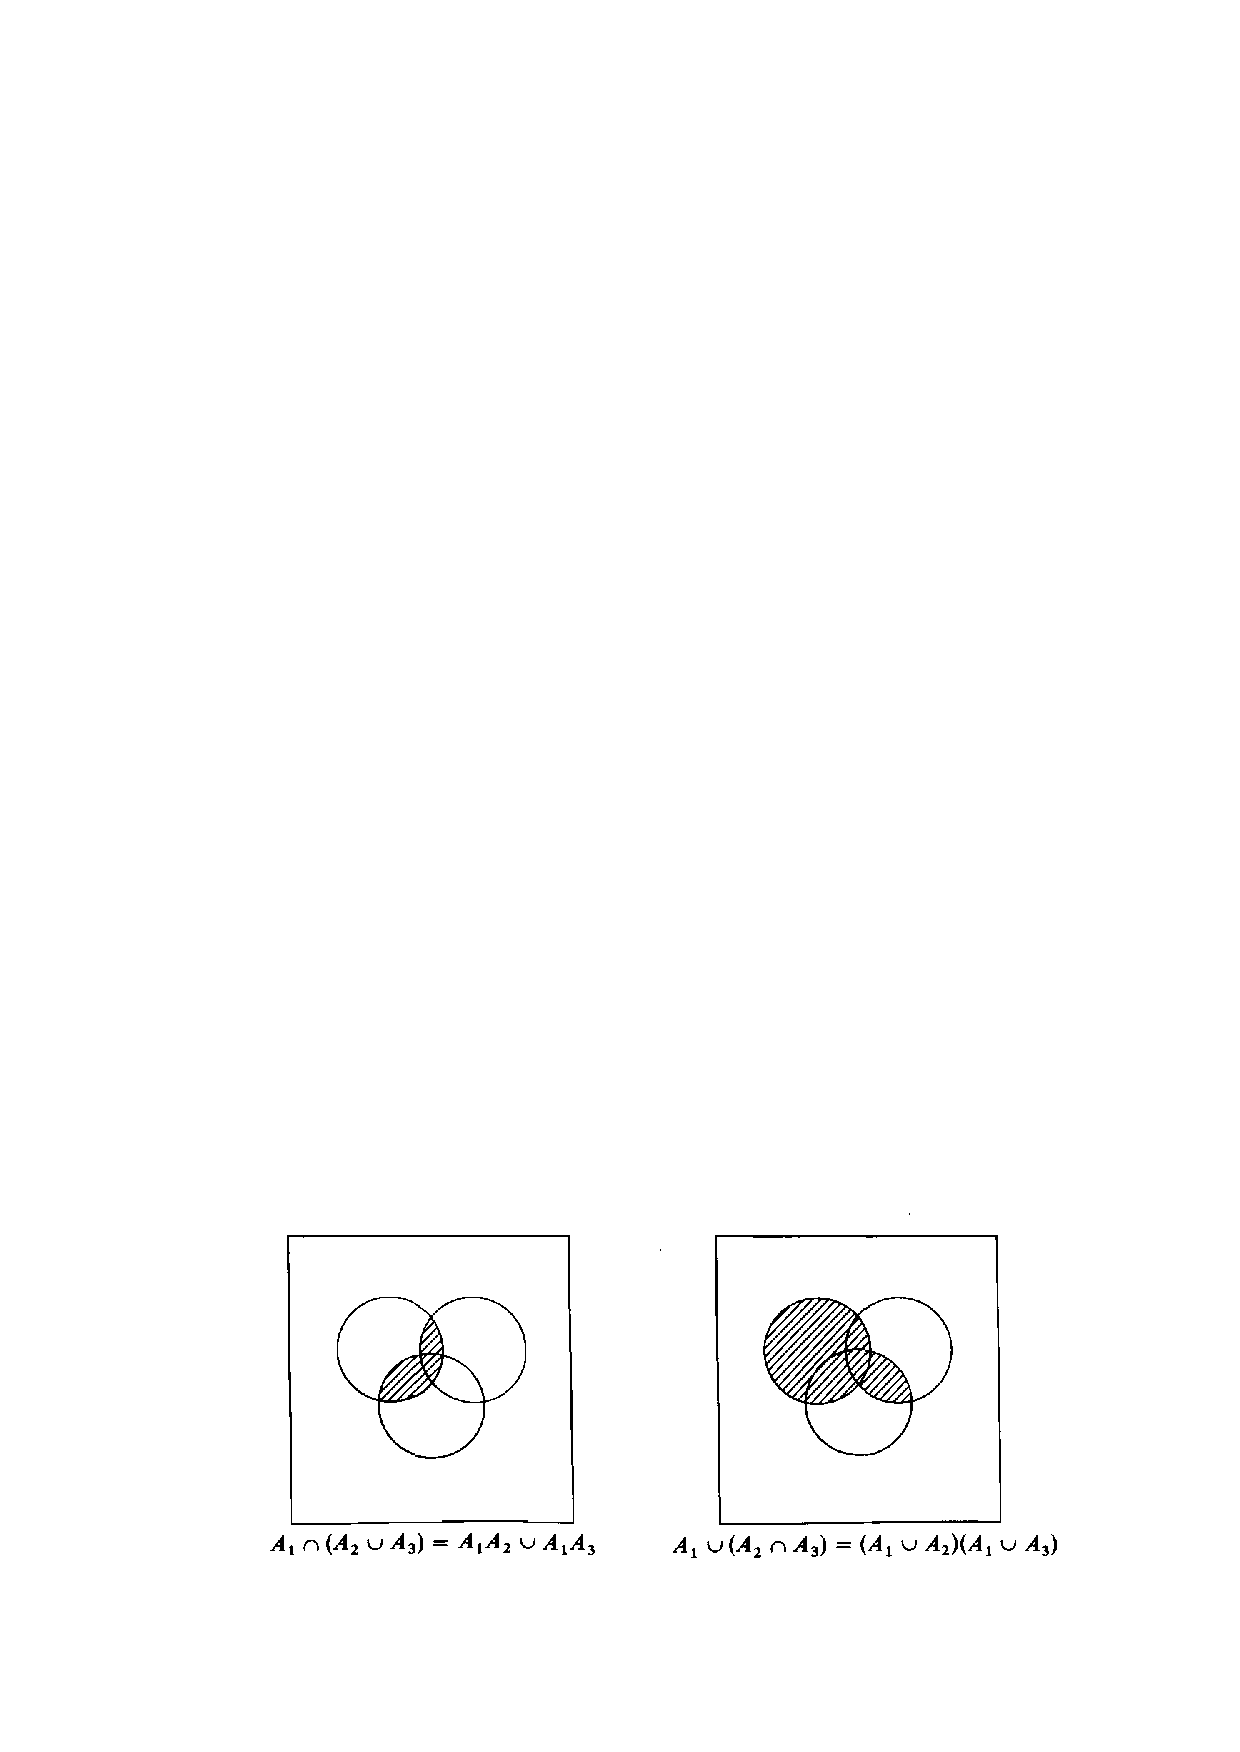
\includegraphics[width=0.9\textwidth,height=0.5\textheight]{commutative.pdf}
\end{figure}
\end{frame}


\begin{frame}
\frametitle{Elements of set theory (Venn diagram)}
%\frametitle{Extra exercise (Venn diagram)}
\begin{tiny}
\begin{exercise}
\def\firstcircle{(3,0) circle (1.5cm)}
\def\secondcircle{(0:5cm) circle (1.5cm)}

\colorlet{circle edge}{blue!50}
\colorlet{circle area}{blue!20}

\tikzset{filled/.style={fill=circle area, draw=circle edge, thick},
    outline/.style={draw=circle edge, thick}}

%Set A or B but not (A and B) also known a A xor B
\hspace{1cm} (i)
\begin{tikzpicture}\centering
    \draw[filled, even odd rule] \firstcircle node {$A$}
                                 \secondcircle node{$B$};
    \node[anchor=south] at (current bounding box.north) {$\overline{A \cap B}$};
\end{tikzpicture}

\hspace{5cm} (ii)
% Set B but not A
\begin{tikzpicture}
    \begin{scope}
        \clip \secondcircle;
        \draw[filled, even odd rule] \firstcircle
                                     \secondcircle node {$B$};
    \end{scope}
    \draw[outline] \firstcircle node {$A$}
                   \secondcircle;
    \node[anchor=south] at (current bounding box.north) {$B - A$};
\end{tikzpicture}
\end{exercise}
\end{tiny}
\end{frame}



\begin{frame}
\frametitle{More on sets}

Events can be represented by means of sets and sets can be either countable or uncountable.

\vspace{0.5cm}


In mathematics, a \color{blue} countable set \color{black} is a set with the same cardinality (number of elements) as some subset of the set of
natural numbers ($\mathbb{N}$). \textit{A countable set is either a finite set or a countably infinite set.} Whether finite or infinite, the elements of a
countable set can always be counted one at a time and, although the counting may never finish, every element of the set is associated with a
natural number --- roughly speaking one can count the elements of the set using $1,2,3,..$ \\

\vspace{0.5cm}

G. Cantor introduced the term countable set, contrasting sets that are countable with those that are \color{blue} uncountable
\color{black} (i.e., nonenumerable or nondenumerable).


\end{frame}


\begin{frame}
\frametitle{More on sets}


\begin{example} [Countable]

\begin{figure}[h!]
\centering
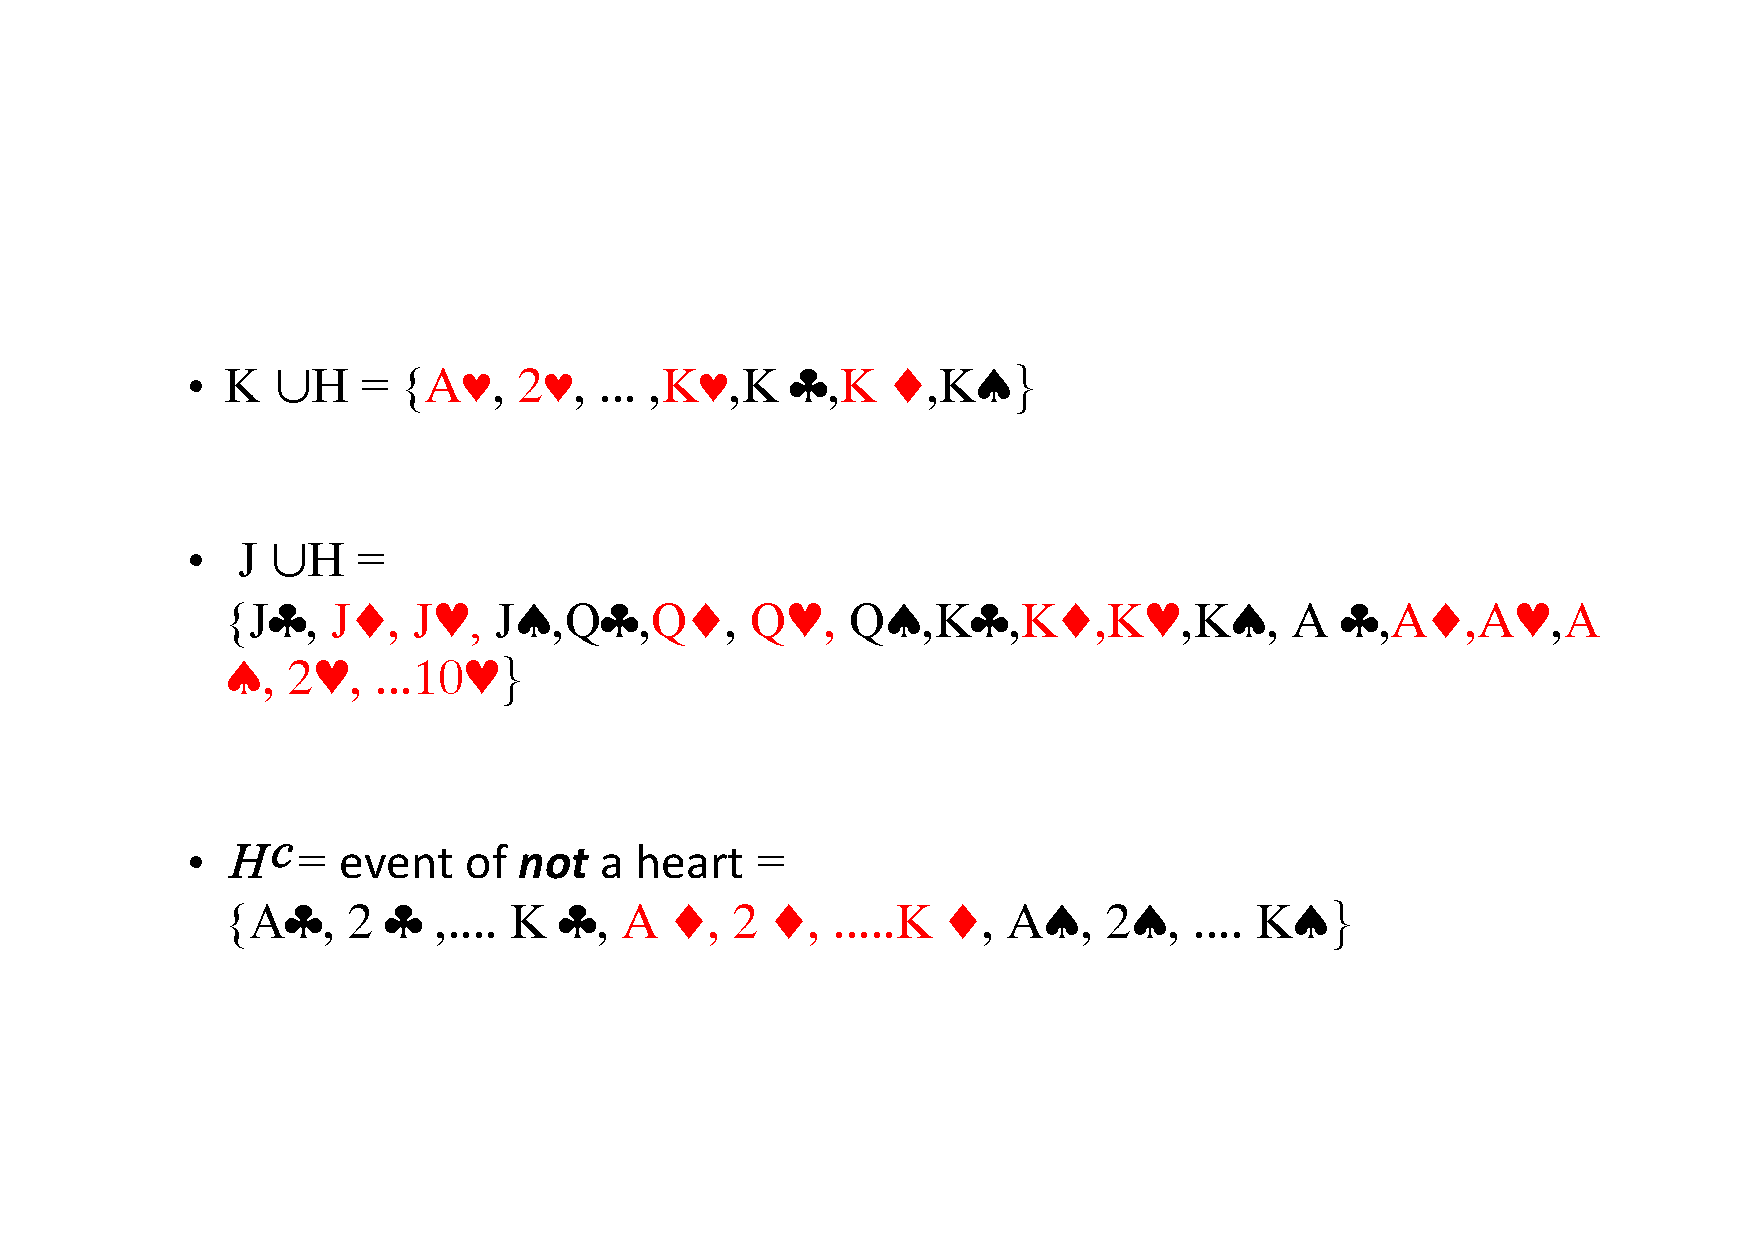
\includegraphics[width=0.9\textwidth,height=0.6\textheight]{Example2.pdf}
\end{figure}


\end{example}

\end{frame}

\begin{frame}
\frametitle{More on sets}

%Events can be represented by means of sets.
\begin{exercise} [Uncountable]
\begin{figure}[h!]
\centering
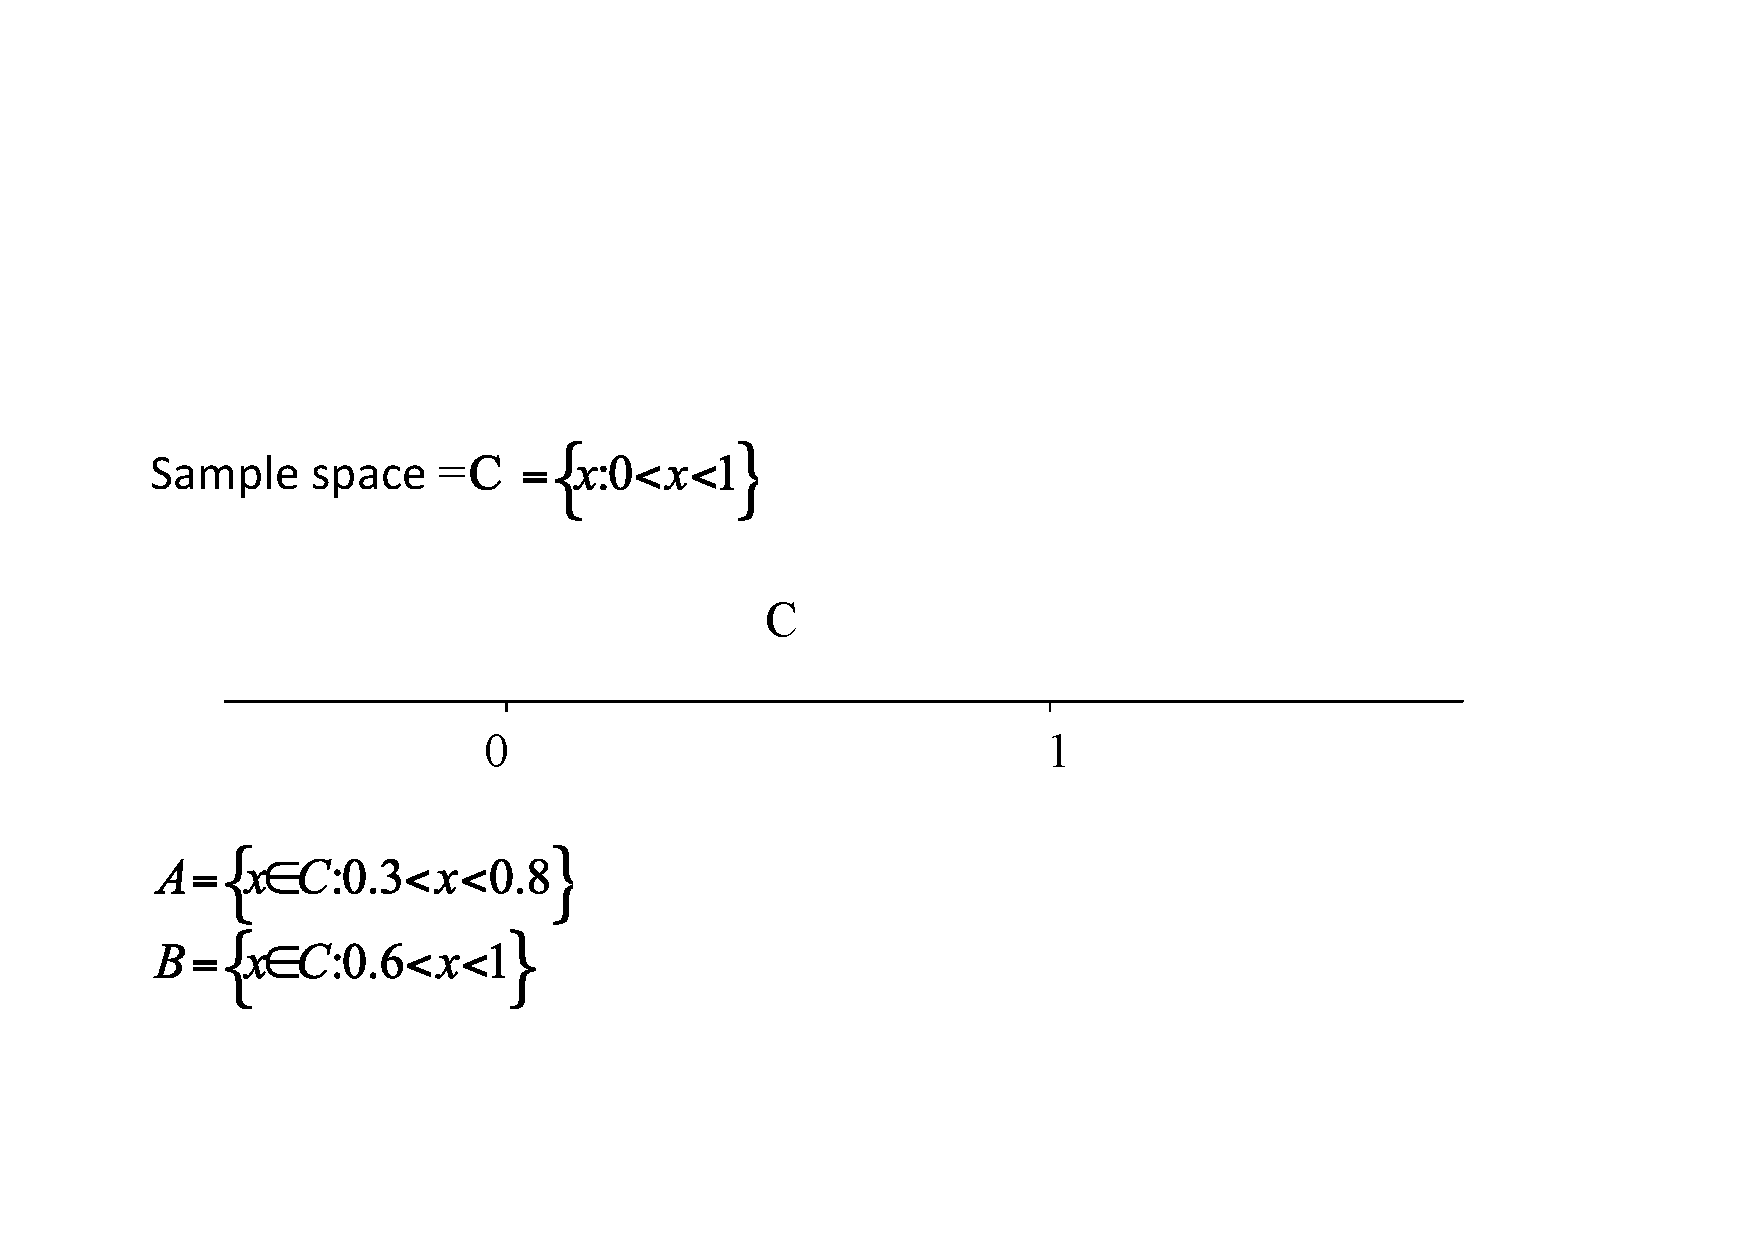
\includegraphics[width=0.9\textwidth,height=0.6\textheight]{Example3.pdf}
\end{figure}
\end{exercise}
\end{frame}


\begin{frame}
\frametitle{More on sets}
\begin{exercise}[cont'd]
and using the definition of $A$ and $B$ compute:
\begin{itemize}
\begin{multicols}{2}
\item $A^c$
\item $B^c$
\item $B^c \cup A$
\item $B^c \cup A^c$
\item $A \cup B$
\item $A \cap B$
\item $B \cup A^c$
\item $A^c \cup A $
\end{multicols}
\end{itemize}

%\begin{figure}[h!]
%\centering
%\includegraphics[width=0.6\textwidth,height=0.6\textheight]{Example3bis.pdf}
%\end{figure}
\end{exercise}
\end{frame}


\begin{frame}
\frametitle{More on sets}
\begin{exercise}[Countable]
Let us consider the  experiment where we flip two coins. For each coin we have $H$ for Head and $T$ for Tail. \\

\vspace{0.5cm}

The sample space (see Lecture 1)
contains the following four points
$$ S = \Big\{ (HH),(HT),(TH),(TT)  \Big\}.$$ \\

\vspace{0.5cm}

Then, let us consider the events:
\begin{itemize}
\item $A= H$ is obtained at least once = $\Big\{ (HH),(HT),(TH) \Big\}$
\item $B=$ the second toss yields $T$ =  $\Big\{ (HT),(TT) \Big\}$
\end{itemize}
%\begin{figure}[h!]
%\centering
%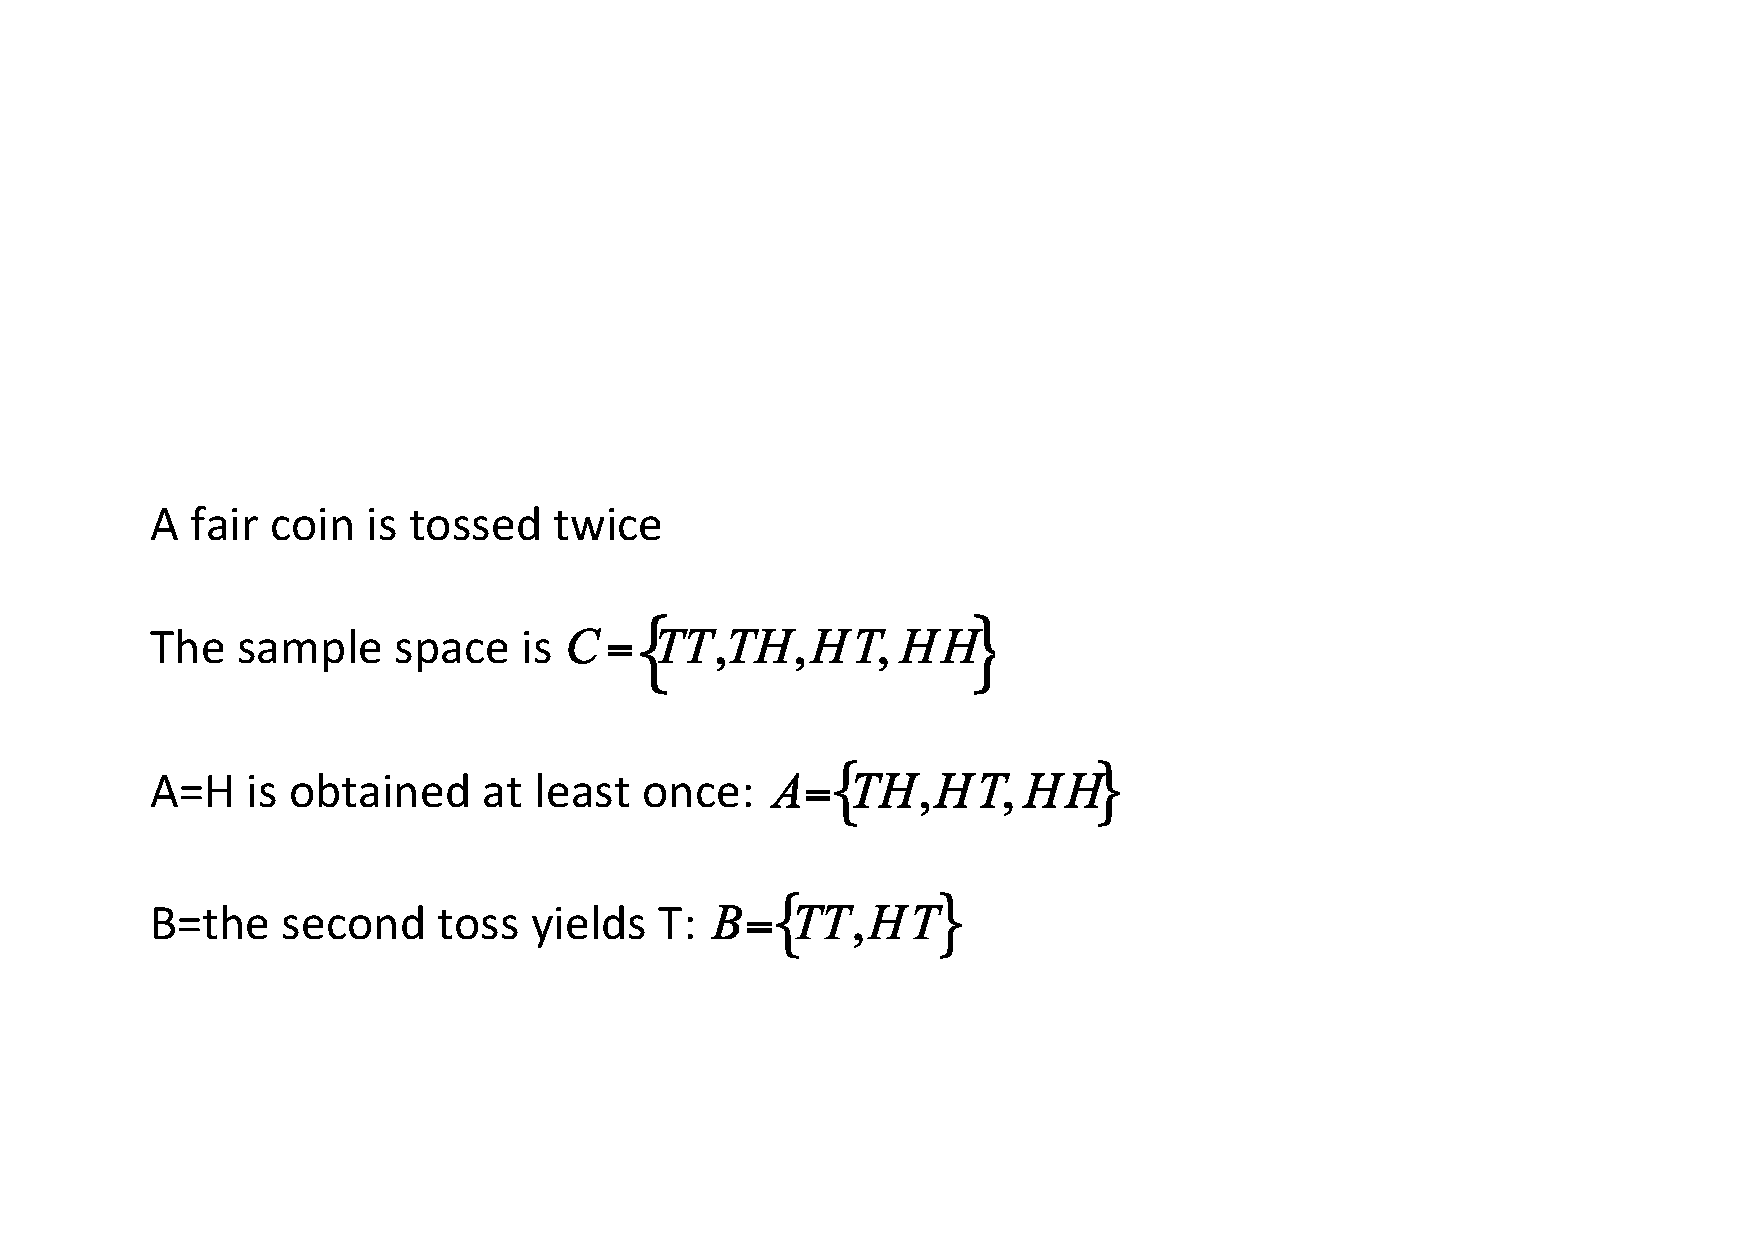
\includegraphics[width=0.9\textwidth,height=0.5\textheight]{Example4.pdf}
%\end{figure}
\end{exercise}
\end{frame}


\begin{frame}
\frametitle{More on sets}
\begin{exercise}[cont'd]
and using the definitions of $A$ and $B$ compute:
%\begin{figure}[h!]
%\centering
%\includegraphics[width=0.8\textwidth,height=0.5\textheight]{Example4bis.pdf}
%\end{figure}
\begin{itemize}
\begin{multicols}{2}
\item $A^c $
\item $B^c$
\item $B^c \cup A$

\item $A \cup B$
\item $A \cap B$
\item $B \cup A^c$
%\item $C^c$
\end{multicols}
\end{itemize}
\end{exercise}

\end{frame}




\begin{frame}
\frametitle{More on sets}
\begin{exercise}[cont'd]
and using the definitions of $A$ and $B$ compute:
%\begin{figure}[h!]
%\centering
%\includegraphics[width=0.8\textwidth,height=0.5\textheight]{Example4bis.pdf}
%\end{figure}
\begin{itemize}
\begin{multicols}{2}
\item $A^c = \{ (TT) \}$
\item $B^c = \{ (HH), (TH) \}$
\item $B^c \cup A$

\item $A \cup B$
\item $A \cap B$
\item $B \cup A^c$
%\item $C^c$
\end{multicols}
\end{itemize}
\end{exercise}

\end{frame}



\begin{frame}
\frametitle{More on sets}

\begin{proposition}
Let $A$ be a set in $S$ and let $\varnothing$ denote the empty set \footnote{A set is called empty if it contains no elements.}. The following relations hold:
\begin{itemize}
\begin{multicols}{2}
\item $A \cap S = A$;
\item $A \cup S = S$;
\item $A \cap \varnothing = \varnothing$;
\item $A \cup \varnothing = A$;
\item $A \cap A^c = \varnothing$;
\item $A \cup A^c = S$;
\item $A \cap A = A$;
\item $A \cup A = A$;
\end{multicols}
\end{itemize}
\end{proposition}
\vspace{0.4cm}
The relations can be verified easily using Venn diagrams ... [do it!]
\end{frame}





\begin{frame}
\frametitle{More on sets}
The above relations are helpful to define some other relations between sets/events.
\begin{example}
Let $A$ and $B$ be two sets in $S$. Then we have
$$
B = (B \cap A) \cup (B \cap A^c).
$$
To check it, we can proceed as follows:
\bea
B & = & S \cap B \nn \\
 & = & (A \cup A^c) \cap B \nn \\
 & = &  (B \cap A) \cup (B \cap A^c). \nn
\eea
That concludes the argument.
\end{example}


\end{frame}


\begin{frame}
\frametitle{De Morgan's Laws: 1\text{st} law}

Let $A$ and $B$ be two sets in $S$. Then:
\bea
(A\cap B)^{c} =A^c \cup B^c,  \nn
\eea

where: \vspace{0.4cm}

\begin{itemize}
\item Left hand side: \color{blue}$(A\cap B)^{c}$ \color{black} represents the \textbf{set of all elements that are not both $A$ and $B$}; \vspace
{0.4cm}
\item Right hand side:  \color{blue}$A^c \cup B^c$ \color{black} represents all elements that are not $A$ (namely they are $A^c$) and not $B
$ either (namely they are $B^c$) $\Rightarrow$ \textbf{set of all elements that are not both $A$ and $B$}.
\end{itemize}
\end{frame}



\begin{frame}
\frametitle{De Morgan's Laws: 2\text{nd} law}

Let $A$ and $B$ be two sets in $S$. Then:
\bea
(A\cup B)^{c} =A^c \cap B^c,  \nn
\eea

where: \vspace{0.4cm}

\begin{itemize}
\item Left hand side: \color{blue}$(A\cup B)^{c}$ \color{black} represents the \textbf{set of all elements that are neither $A$ nor $B$}; \vspace
{0.4cm}
\item Right hand side:  \color{blue}$A^c \cap B^c$ \color{black} represents the intersection of all elements that are not $A$ (namely they are $A^c$) and not $B
$ either (namely they are $B^c$) $\Rightarrow$ \textbf{set of all elements that are neither $A$ nor $B$}.
\end{itemize}
\end{frame}


\begin{frame}
\frametitle{De Morgan's Theorem}
More generally, we can consider unions and intersections of many (countable) sets. So, we state the general results,
\begin{theorem} [De Morgan]
Let $\mathbb{N}$ be the set of natural number and $\{A_{i}\}$ a collection (indexed by $i \in \mathbb{N}$) of subsets of $S$. Then:
\begin{itemize}
\item[(i)]
\bea
\overline{\bigcup_{i \in \mathbb{N}} A_i} &=& \bigcap_{i \in \mathbb{N}} \overline{A}_i;
\eea
\item[(ii)]
\bea
\overline{\bigcap_{i \in \mathbb{N}} A_i} &=& \bigcup_{i \in \mathbb{N}} \overline{A}_i.
\eea

\end{itemize}
\end{theorem}
\end{frame}

%\begin{frame}
%\frametitle{Back to the events}
%
%
%The sample space of an experiment is denoted by $S$ and it is the complete listing of the elementary events (which are representable by means of
%sets) associated to a random experiment.
%\begin{example} [Countable]
%\begin{figure}[h!]
%\centering
%\includegraphics[width=0.8\textwidth,height=0.6\textheight]{Example11.pdf}
%\end{figure}
%\end{example}
%
%
%\end{frame}


\begin{frame}
\frametitle{Back to the events}

\textbf{Our primary interest will be not in events per se, but it will be in the \color{blue}\textit{probability that an event does or does not happen}.}
 \color{black} \\ \vspace{0.2cm}

Intuitively,
the probability of an event is the number  associated to the event:
$$
\text{event} \rightarrow \text{pr(event)}
$$
such that:
\begin{enumerate}
\item the probability is positive or more generally non-negative (it can be zero);
\item the $\text{pr}(S)=1$ (remember, $S$ is the sample space) and $\text{pr}(\varnothing)=0$;
\item the probability of two (or more) mutually exclusive events is the sum of the probabilities of each event.
\end{enumerate}



\end{frame}



\begin{frame}
\frametitle{Back to the events}

In many experiments, it is natural to assume that all outcomes in the sample space ($S$) are equally likely to occur. That is, consider an experiment whose sample space is a finite set, say, $S=\{1,2,3,...N\}$. Then, it is often natural to assume that
\bea
P(\{1\})=P(\{2\})=...=P(\{N\}) \nonumber
\eea
or equivalently $P(\{i\})= 1/N$, for $i=1,2,...,N$. \\
\vspace{0.5cm}
Now, if we define a composite event $A$, there exist $N_A$ realizations having the same likelihood (namely, the have the same
probability) in the event $A$, so
$$
\boxed{P(A)=\frac{N_A}{N}=\frac{\mbox{\# of favorable outcomes}}{\mbox{total \# of outcomes}}=\frac{\mbox{\# of outcomes in $A$}}{\mbox{ \# of outcomes in $S$}}}
$$


where the notation $\# $ means ``number''.

\end{frame}


\begin{frame}
\frametitle{Back to the events}

\begin{example}

We roll a fair die and we define the event $$A=\text{the outcome is an even number}=\{2,4,6\}.$$
What is the probability of $A$?
\vspace{0.5cm}

First, we identify the sample space as
$$S=\{1,2,3,4,5,6\}.$$
Then,
%since the die is fair, each outcome is equally
%likely, so
%\bea
%\text{pr}(\{1\})=\text{pr}(\{2\})=...=\text{pr}(\{6\})=\frac{1}{6}. \nonumber
%\eea
%Thus, we conclude that
we have that
$$
P(A)=\frac{N_A}{N} = \frac{\mbox{3 \text{favorable outcomes}}}{\mbox{6 total outcomes}} = \frac{1}{2}. %= \text{pr}(\{1\})+\text{pr}(\{2\})+\text{pr}(\{3\})
$$


\end{example}


\end{frame}


\begin{frame}
\frametitle{Back to the events}

Building on the intuition gained in the last example (see boxed formula), we state a first \color{blue} informal \color{black} definition
of probability. Specifically, one way of defining the probability of an event is in terms of \textit{relative frequency}.

\begin{definition}[Informal]
Suppose that an experiment, whose sample space is $S$, is repeatedly performed under exactly the same conditions. For each event, say $A$, of the sample space, we define $n(A)$ to be the number of times in the first $n$ repetitions of the experiment that the event $A$ occurs. Then, $P(A)$, namely the probability of the event $A$, is defined as:
$$
P(A)=\lim_{n \to \infty} \frac{n(A)}{n},
$$

that is $P(A)$ is defined as the limiting proportion/frequency of time that $A$ occurs: it is the limit of relative frequency of $A$.
\end{definition}



\end{frame}

\begin{frame}
\frametitle{Back to the events}
\begin{example}[Tossing a well-balanced coin]
In tossing a well-balanced coin, there are 2 mutually exclusive equiprobrable outcomes: H and T. Let $A$
be the event of head (H). Since the coin is fair, we have $P(A)=1/2$. To confirm this intuition/conjecture we can toss the coin a large number of times (each under identical conditions) and count the times we have H. Let $n$ be the \textbf{total \# of repetitions} while $n(A)$ is the \textbf{\# of times in which we observe $A$}. Then, the relative frequency:
$$
\lim_{n \to \infty} \frac{n(A)}{n},
$$
converges to $P(A)$. So,
$$
P(A) \sim \frac{n(A)}{n}, \quad \text{for large $n$}.
$$

\end{example}
\end{frame}


\begin{frame}
\frametitle{Back to the events}
\begin{example}[cont'd]

\begin{figure}[h!]
\centering
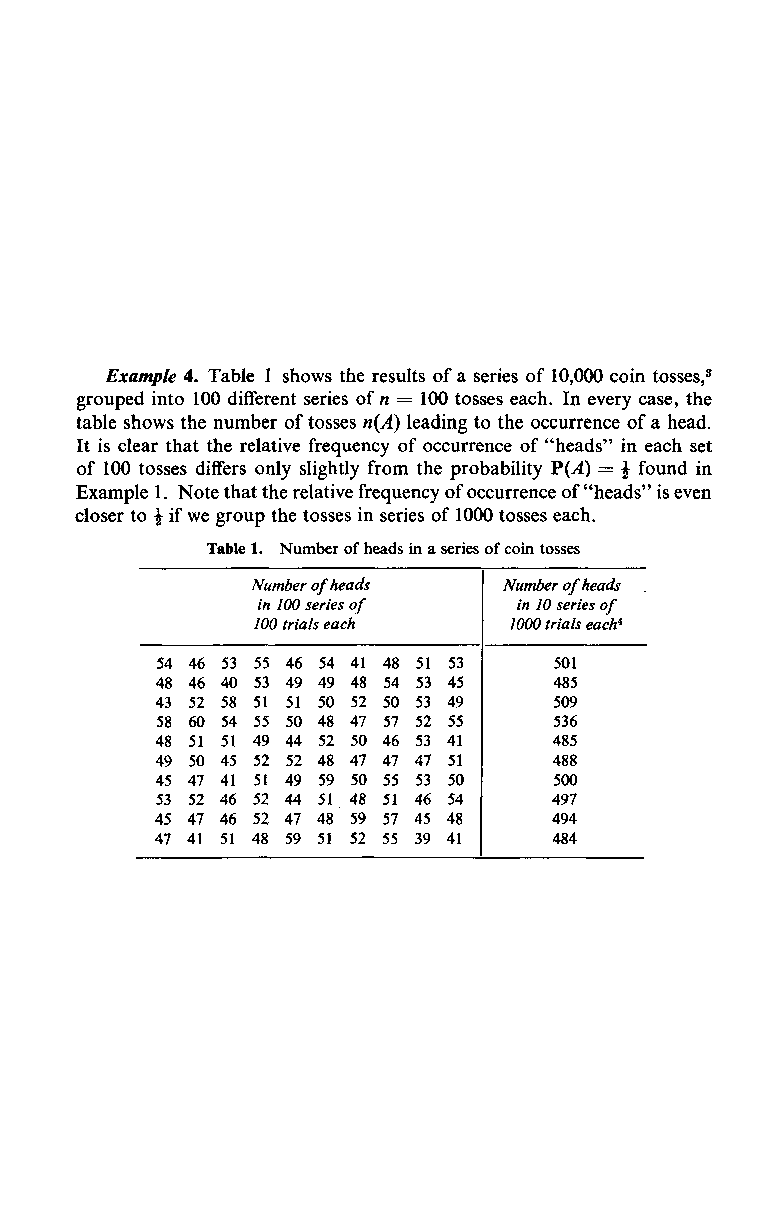
\includegraphics[width=0.7\textwidth,height=0.7\textheight]{roz.pdf}
\end{figure}



\end{example}
\end{frame}
%
%\begin{frame}
%\frametitle{Back to the events}
%
%Clearly,
%$$0 \leq n(A) \leq n, \quad \text{so} \quad  0 \leq P(A) \leq 1.$$
%Thus, we say that  \color{blue} the probability is a set function (it is defined on sets) and it associates to each set/event a number between zero and one.
%\color{black}
%
%\vspace{0.5cm}
%
%Now, let us recall that a real-valued function is a mapping from $D_f$ to $\mathbb{R}$ and we write:
%$$
%f \quad : \quad D_f \to \mathbb{R},
%$$
%where $D_f$ is the domain of $f$ and $\mathbb{R}$ is the range. \\
%
%\vspace{0.5cm}
%
%\color{red} \textbf{Q.} \color{black} In the case of the (function) probability, we already know that the range is $[0,1]$, but what about $D_f$?
%
%\end{frame}
%
%
%
%\begin{frame}
%\frametitle{Back to the events}
%
%To define $D_f$ for
%the probability, we have to rely on the set theory --- indeed $D_f$ has to be related to sets/events. To this end,
%%\vspace{0.3cm}
%\begin{definition} [$\sigma$-algebra]
%The $\sigma$-algebra $\mathcal{B}$ generated by the sample space $S$ is defined as the collection of all subsets of $S$ satisfying:
%\begin{enumerate}
%\item[(i)] $S \in \mathcal{B}$;
%\item[(ii)] if $A \in \mathcal{B}$, then $A^c \in \mathcal{B}$;
%\item[(iii)] if $A_1 \in \mathcal{B}$ and $A_2 \in \mathcal{B}$, then $A_1 \cup A_2 \in \mathcal{B}$. More generally, for a collection of events $\{A_i\}$, with $i \in \mathbb{N}$, we have
%\bea
%A = \bigcup_{i \in \mathbb{N}} A_i \text{ \ is such that \ }  A \in \mathcal{B}. \nn
%\eea
%
%\end{enumerate}
%\end{definition}
%
%Thus,  we will have that
%$$
%\boxed{P \quad : \quad \mathcal{B} \to [0,1]. }
%$$
%
%\end{frame}
%
%
%\begin{frame}
%\frametitle{Back to the events}
%
%%In this way, we define the domain of the probability. Then,
%To provide a formal definition of probability, we will make use of $\mathcal{B}$ and we will need to impose some additional conditions (that we are going to call \textit{axioms}). \\
%\vspace{0.5cm}
%We here briefly state the ideas, then we will formalize them: \\
%\vspace{0.3cm}
%(i) When we define the probability we would want the have a domain (namely $\mathcal{B}$) such that it includes the
%sample space $S$, and $P(S)=1$. \\ \vspace{0.1cm}
%(ii)  Moreover, for the sake of completeness, if $A$ is an event and we can talk about the probability that $A$ happens, then it is
%suitable for us that $A^c$ is also an event in $\mathcal{B}$, so that we can talk about the probability that $A$ does not happen. \\ \vspace{0.1cm}
%(iii) Similarly, if
%$A_1$ and $A_2$ are two events (so we can say something about their probability of happening), so we should be able to say something about the probability of the event $A_1 \cup A_2$.
%
%
%\end{frame}




\begin{frame}
\frametitle{Back to the events}

Clearly,
$$0 \leq n(A) \leq n, \quad \text{so} \quad  0 \leq P(A) \leq 1.$$
Thus, we say that  \color{blue} the probability is a set function (it is defined on sets) and it associates to each set/event a number between zero and one.
\color{black}

\vspace{0.15cm}
\begin{remark}
One can provide a more rigorous definition of probability, as a real-valued function which defines a mapping between sets/events and the interval $[0,1]$. To achieve this goal one needs the concept of sigma-algebra (which represents the domain of the probability), but we do not pursue with that---at the cost of losing the mathematical rigour of the next slide!!
\end{remark}

\end{frame}



\begin{frame}
\frametitle{Back to the events}

%In this way, we define the domain of the probability. Then,
To express the probability,  we need to impose some additional conditions, that we are going to call \textbf{\textit{axioms}}. \\
\vspace{0.5cm}
We here briefly state the ideas, then we will formalize them: \\
\vspace{0.3cm}
(i) When we define the probability we would want the have a domain such that it includes the
sample space $S$ and $P(S)=1$. \\ \vspace{0.1cm}
(ii)  Moreover, for the sake of completeness, if $A$ is an event and we can talk about the probability that $A$ happens, then it is
suitable for us that $A^c$ is also an event, so that we can talk about the probability that $A$ does not happen. \\ \vspace{0.1cm}
(iii) Similarly, if
$A_1$ and $A_2$ are two events (so we can say something about their probability of happening), so we should be able to say something about the probability of the event $A_1 \cup A_2$.


\end{frame}



\begin{frame}
\frametitle{Some references}

%The interested Student can find some additional info in the books: \\

\vspace{1.5cm}
\begin{itemize}
\item \textit{Introduction to mathematical statistics}, Hogg, McKean, and Craig, 7th edition (2013), Ed: Pearson.
\vspace{0.25cm}
\item \textit{Probability theory: a coincise course}, Rozanov, 3rd edtion (1969), Ed: Dover Publication.
\end{itemize}

\end{frame}
%
%
%\begin{frame}
%\frametitle{Back to the events}
%
%%Beyond the mathematical formalism, the interpretation of $\mathcal{B}$ goes like that:
%%\begin{interpretation}
%We said earlier that we are not interested in the events per se mainly because our focus is on the \textbf{probability} that an event happens.
%As we said, the \textbf{probability is a function}. Now,  any function is a rule (law, formula, recipe) that associates each point in one set of points (the
%domain) with one and only one point in another set of points (range). \\ \vspace{0.2cm}
%
%
%(i) When we define the probability we would want the have a domain (namely $\mathcal{B}$) such that it includes the
%sample space $S$. \\ \vspace{0.1cm}
%(ii)  Moreover, for the sake of completeness, if $A$ is an event and we can talk about the probability that $A$ happens, then it is
%suitable for us that $A^c$ is also an event in $\mathcal{B}$ so that we can talk about the probability that $A$ does not happen. \\ \vspace{0.1cm}
%(iii) Similarly, if
%$A_1$ and $A_2$ are two events (so we can say something about their probability of happening), so should $A_1 \cup A_2$ be an event too.
%%\end{interpretation}
%
%
%\end{frame}




\end{document}

